\documentclass[a4paper, 12pt]{report}

%%%%%%%%%%%%
% Packages %
%%%%%%%%%%%%

\usepackage[spanish]{babel}
\usepackage{packages/sleek}
\usepackage{packages/sleek-title}
\usepackage{packages/sleek-theorems}
\usepackage{packages/sleek-listings}
\usepackage{dirtree}
\usepackage{tikz}
\usepackage{pgfplots}
\usepackage{pgfplotstable}
\usepackage{tikz}
\usetikzlibrary{automata} % Carga la librería automata




%%%%%%%%%%%%%%
% Title-page %
%%%%%%%%%%%%%%

\logo{./resources/pdf/logo.pdf}
\institute{Universidad Politécnica de Cartagena}
\faculty{Ingeniería Telemática}
%\department{Department of Anything but Psychology}
\title{Conexión Cliente-Servidor mediante sockets en Java}
\subtitle{Trabajo de prácticas de sistemas distribuidos }
\author{\textit{Autores}\\\textsc{Álvaro Herández Riquelme}\\ y \textsc{André Yermak Naumenko}}
%\supervisor{Linus \textsc{Torvalds}}
%\context{A long time ago in a galaxy far, far away...}
\date{\today}

%%%%%%%%%%%%%%%%
% Bibliography %
%%%%%%%%%%%%%%%%

\addbibresource{./resources/bib/references.bib}

%%%%%%%%%%
% Macros %
%%%%%%%%%%

\def\tbs{\textbackslash}

%%%%%%%%%%%%
% Document %
%%%%%%%%%%%%

\begin{document}
    \maketitle
    \romantableofcontents

\newpage

    \chapter{Introducción}

    En este documento se presenta el trabajo realizado en la asignatura de sistemas distribuidos, en el cual se ha
    implementado un sistema de transferencia de archivos entre un cliente y un servidor mediante sockets en Java.
    Se ha elegido el uso de sockets para la comunicación entre el cliente y el servidor, ya que lo consideramos una
    forma más sencilla y eficiente de implementar lo que se pide en estre trabajo.

    \section{Estructura del proyecto}

    La estructura del proyecto se basa mayoritariamente alrededor de \textbf{la máquina de estados} que hemos
    diseñado para éste, siendo de gran importancia el contexto que tenga el programa en todo momento, ya sea
    cliente, servidor, o system, el contexto que tiene la máquina antes de poder pasar al contexto de cliente o
    servidor.
%
%    \begin{figure}[htb]
%        \centering
%        \begin{tikzpicture}[]
%            \node[state] (s1) {Sistema};
%            \node[state, below right of=s1] (s2) {Cliente};
%            \node[state, below left of=s1] (s3) {Servidor};

%            \draw
%            (s1) edge[bend left]    (s2)
%            (s1) edge[bend right]   (s3)
%            (s2) edge[bend left]    (s1)
%            (s3) edge[bend right]   (s1);
%        \end{tikzpicture}
%        \caption{Máquina de estados diseñada para el proyecto.}
%        \label{fig:diagrama}
%    \end{figure}

    \begin{figure}[H]
        \centering
        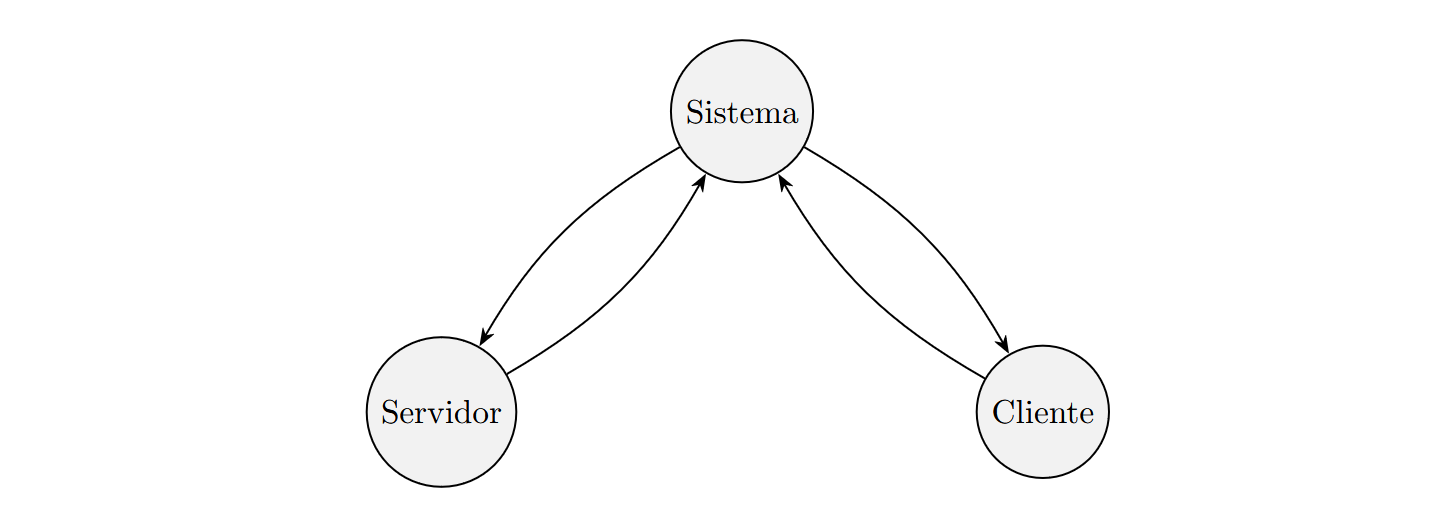
\includegraphics[scale=0.20]{resources/img/diagrama.png}
        \caption{Máquina de estados diseñada para el proyecto.}
        \label{fig:main}
    \end{figure}


    Teniendo en cuenta la maquina de estados (funciona tal tal....), la estructura de archivos finalmente quedará
    organizada de la siguiente manera:

    \dirtree{%
        .1 filetransfer.
        .2 FileSystem.java.
        .2 Main.java.
        .2 SystemContextHandler.java.
        .2 client.
        .3 ClientContextHandler.java.
        .3 ClientMain.java.
        .3 ClientUtils.java.
        .3 SimpleClient.java.
        .2 common.
        .3 CloseMessage.java.
        .3 CommandMessage.java.
        .3 ConsoleGUI.java.
        .3 Const.java.
        .3 Context.java.
        .3 ContextCommandHandler.java.
        .3 ContextManager.java.
        .3 ContextObserver.java.
        .3 Header.java.
        .3 TextMessage.java.
        .3 UserMessage.java.
        .3 Utils.java.
        .2 META-INF.
        .3 MANIFEST.MF.
        .2 server.
        .3 ConcurrentServer.java.
        .3 ServerCommandProcess.java.
        .3 ServerContextHandler.java.
        .3 ServerMain.java.
    }


    \chapter{filetransfer}
    \section{FileSystem.java}
    \section{Main.java}
    \section{SystemContextHandler.java}

    \chapter{common}
    \section{CloseMessage.java}
    \section{CommandMessage.java}

    Comandos disponibles:

    \begin{itemize}
        \item \texttt{FILE\_UPLOAD}
        \item \texttt{FILE\_DOWNLOAD}
        \item \texttt{DIRECTORY\_CREATE}
        \item \texttt{DIRECTORY\_LIST}
        \item \texttt{DIRECTORY\_LOCATION}
        \item \texttt{FILE\_DELETE}
        \item \texttt{DIRECTORY\_OPEN}
        \item \texttt{CON\_CHECK}
    \end{itemize}

    \section{ConsoleGUI.java}
    \section{Const.java}
    \section{Context.java}
    \section{ContextCommandHandler.java}
    \section{ContextManager.java}
    \section{ContextObserver.java}
    \section{Header.java}
    \section{TextMessage.java}
    \section{UserMessage.java}
    \section{Utils.java}

    \chapter{client}
    \section{ClientContextHandler.java}
    \section{ClientMain.java}
    \section{ClientUtils.java}
    \section{SimpleClient.java}

    \chapter{server}

    \section{ServerMain.java}

    Al inicio del contexto en el servidor, se crea una instancia de \text{ServerMain}, que actúa como el punto de
    entrada principal para iniciar un servidor de transferencia de archivos. La clase extiende ContextManager,
    por lo que hereda funcionalidades relacionadas con la gestión del contexto. Al instanciarse, ServerMain recibe
    un puerto como parámetro y utiliza métodos de la clase Utils (getPublicIP() y getPrivateIP())
    para obtener tanto la dirección IP pública como la privada del
    servidor. Estas direcciones IP se almacenan en variables de instancia y se muestran por consola cuando el servidor se inicia.

    El método start()
    es el encargado de iniciar el servidor. Primero, imprime un mensaje
    indicando que el servidor ha comenzado a escuchar en el puerto
    especificado, junto con las direcciones IP pública y privada. Luego,
    crea una instancia de ConcurrentServer, pasando el puerto y la propia instancia de ServerMain (que actúa como ContextManager) como argumentos. Finalmente, llama al método run() de ConcurrentServer,
    lo que inicia el servidor concurrente y comienza a aceptar conexiones
    de clientes. Este diseño permite que el servidor maneje múltiples
    conexiones de manera eficiente, utilizando un pool de hilos para
    gestionar cada cliente de forma independiente.



    \section{ConcurrentServer.java}

    El concurrentserver, cuyo nombre viene dado por las prácticas aunque se haya modificado, manejará múltiples
    conexiones de clientes utilizando un pool de hilos. Cuando el servidor se inicia, escucha en un puerto
    específico y declara un \texttt{ExecutorService}  con un número fijo de hilos definido por
    \texttt{Const.MAX\_THREADS}. El servidor entra en un bucle infinito donde espera conexiones de clientes. Cada
    vez que un cliente se conecta, se crea obtiene un \texttt{Socket} que
    representa la conexión con ese cliente y muestra la dirección del cliente
    conectado. Para manejar la conexión, el servidor crea un nuevo hilo en el pool de hilos, donde se instancia un
    objeto \texttt{SimpleServer} pasándole el socket del cliente y se llama al método `run()`. Este método es el
    encargado de gestionar la comunicación con el cliente. De esta forma que el servidor atienda a varios
    clientes de manera simultánea.

    \section{ServerCommandProcess.java}

    El ServerCommandProcess, es el encargado de procesar los objetos \textbf{CommandMessage} que recibe el
    servidor, y actuar en consecuencia. Cada comando requiere una función propia, y al optar
    por hacerlo con un enfoque distinto al de clase, donde cada comando podría ser una clase distinta y que cada
    función se ejecute según el objeto, se ha hecho un \textbf{hashmap} que contiene las funciones que se ejecutarán
    según el comando que se reciba.

    Todas las funciones que se ejecutan en el hashmap, reciben un objeto de tipo cm,
    que será el comando enviado por el cliente, ya habiendo pasado las validaciones tanto de tipado (el casting),
    como de argumentos (En la parte del cliente). Cada función del hashmap también recibe un objeto de tipo
    \textbf{Path}, del paquete de java.nio, que será el directorio en el que se ejecutará el comando, el cual se
    procesa al inicio de la clase. Este path es una combinación del basepath, donde se encontrará storage, y el
    clientpath, que será el directorio en el el servidor entiende que se encuentra el cliente. La función
    \textbf{directoryOpen} es la que actualiza el clientpath, y se ejecuta cuando el comando del cliente es
    \textbf{cd}. Se tiene en cuenta que el cliente no pueda salir del directorio base.

    \section{ServerContextHandler.java}

    El serverContextHandler hace función similar que el clientContextHandler, pero en menor medida, ya que el
    dispositivo que actúa como servidor no tiene que enviar muchos comandos, por lo que tiene comandos basicos como
    --close o --help


\end{document}
